\pagina{Resultados experimentales}
\subsection{Balance acumulado de todas las entregas}
Se evaluaron 149 grafos distintos entre la evaluación distribuida y las dos exploraciones cerradas. De ellos, \UnionCertifiedGraphs{} tienen ciclo certificado: 15 de la evaluación distribuida, dos de la exploración guiada y cinco de la reparación v4. La figura~\ref{fig:cumulativecoverage} presenta esa cobertura acumulada por familia; el cuadro~\ref{tab:solved} y la figura~\ref{fig:heatmap} incluyen los 22 grafos. Las tasas y los tiempos de cada protocolo se analizan después con sus respectivos presupuestos.

\begin{figure}[H]\centering
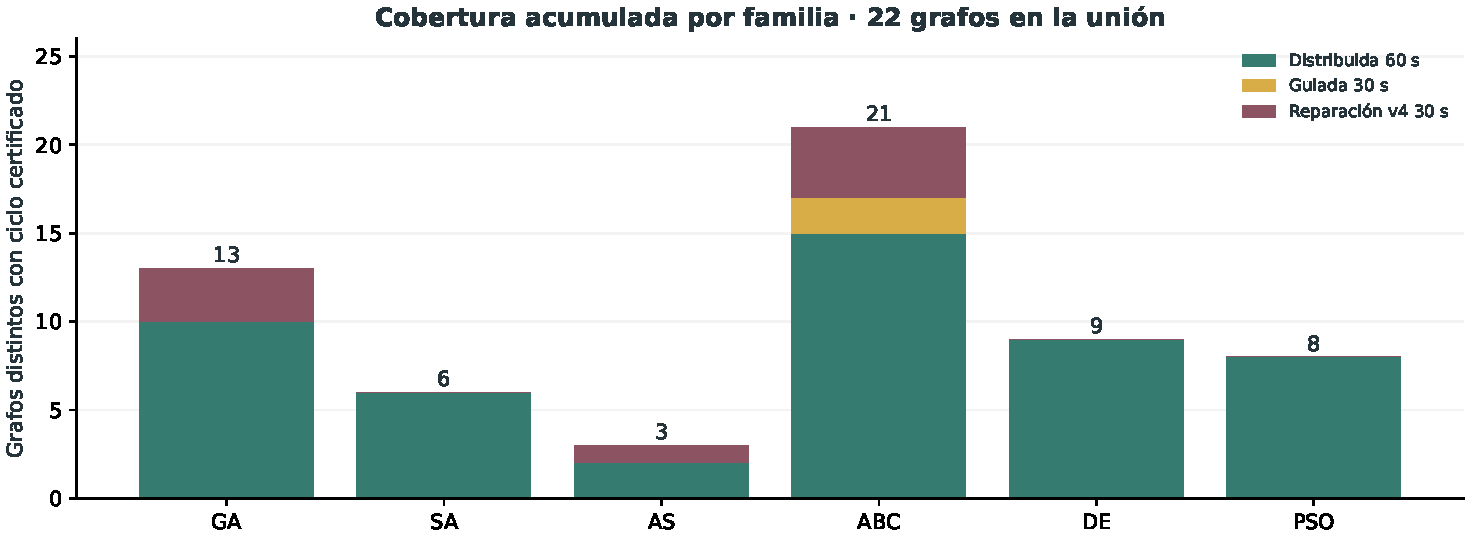
\includegraphics[width=\linewidth]{figures/exploratory-cumulative-coverage.pdf}
\caption{Grafos distintos certificados por familia a lo largo de las tres entregas. Cada color identifica el protocolo que añade el certificado. Las familias pueden resolver el mismo grafo: las barras se solapan en cobertura y no se suman para obtener los 22 grafos de la unión. No es una comparación de tasas ni tiempos entre protocolos.}\label{fig:cumulativecoverage}
\end{figure}

\subsection{Campaña inicial: límites observados}
La campaña inicial registró cero ciclos certificados en los 900 primarios de evaluación y escala, distribuidos en 150 intentos por familia. Hubo 630 agotamientos por plazo y 270 por evaluaciones, sin errores de ejecución ni timeouts externos en esos primarios. En 30 intentos de AS sobre graph1001 no se completó candidato y no se asignó costo ficticio.

\begin{table}[H]\centering\small
\caption{Resultados principales de la campaña histórica M6. Los límites efectivos son motivos de parada, no una prueba de imposibilidad.}\label{tab:historical}
\begin{tabularx}{\linewidth}{Yrrrr}
\toprule
Familia & Éxitos/150 & Plazos & Eval. límite & Sin candidato \\ \midrule
GA & 0/150 & 90 & 60 & 0 \\
SA & 0/150 & 90 & 60 & 0 \\
AS & 0/150 & 150 & 0 & 30 \\
ABC & 0/150 & 60 & 90 & 0 \\
DE & 0/150 & 120 & 30 & 0 \\
PSO & 0/150 & 120 & 30 & 0 \\
\bottomrule\end{tabularx}

\end{table}

AS mostró un cuello de botella de construcción: en la instancia de escala no terminó rutas completas. En graph48, las otras cinco familias alcanzaron las 10\,000 evaluaciones en todos los intentos; en graph479 y graph1001 todas las familias llegaron al plazo temporal. Un presupuesto máximo común no produjo el mismo número de evaluaciones efectivas. Las incidencias de swap y alimentación se preservaron en la campaña y limitaron las conclusiones temporales.

No existe un ganador por éxito en esta etapa. La coincidencia de los seis pares de verificación sustenta la reproducibilidad de rutas, costos, estados y contadores bajo su protocolo; no exige ni implica tiempos idénticos.

\subsection{Cobertura y resultados de la evaluación final}
La evaluación consolidada registra \TotalAttempts{} intentos: \TotalSuccesses{} éxitos certificados, \TotalExhausted{} agotamientos y \TotalErrors{} incidencias. La tasa descriptiva conjunta es \SuccessRate\%, incluidos los errores. Los éxitos corresponden a \SolvedGraphs{} grafos distintos, no a \TotalSuccesses{} grafos.

\begin{table}[H]\centering\small
\caption{Entrega por integrante. ``Completos'' indica 60 combinaciones conciliadas, no grafos resueltos. HC indica grafos distintos certificados.}\label{tab:members}
\begin{tabularx}{\linewidth}{Yrrrrr}
\toprule
Equipo & Intentos & Completos & Parciales & HC & Éxitos \\ \midrule
Arturo & 2\,417 & 40 & 1 & 4 & 72 \\
Elías & 600 & 10 & 0 & 1 & 13 \\
Eder & 2\,611 & 42 & 2 & 4 & 98 \\
Zapata & 1\,325 & 22 & 1 & 3 & 72 \\
César & 1\,853 & 30 & 1 & 3 & 90 \\
\bottomrule\end{tabularx}

\end{table}

De los 1001 candidatos, 852 no se iniciaron en las entregas. Entre los 149 iniciados se resolvieron 15 (10.07\%); este porcentaje describe el corte, no la probabilidad de resolver un grafo aleatorio del challenge. Los cinco parciales se mantienen identificados en el cuadro~\ref{tab:partial}.

\begin{table}[H]\centering\small
\caption{Grafos con cobertura parcial al cierre.}\label{tab:partial}
\begin{tabularx}{\linewidth}{lYrrr}
\toprule
Grafo & Equipo & Intentos & Pendientes & Incidencias \\ \midrule
104 & Zapata & 5 & 55 & 1 \\
153 & César & 53 & 7 & 1 \\
185 & Arturo & 17 & 43 & 1 \\
222 & Eder & 48 & 12 & 0 \\
227 & Eder & 43 & 17 & 0 \\
\bottomrule\end{tabularx}

\end{table}

\subsection{Comparación entre las seis familias}
El cuadro~\ref{tab:algorithms} restringe la comparación a los 144 grafos con cobertura completa. Todos los éxitos del corte se encuentran en ese grupo. El denominador es 1\,440 intentos por algoritmo; las nueve incidencias de ese grupo se conservan. Las tres incidencias restantes pertenecen a grafos parciales.

\begin{table}[H]\centering\small
\caption{Resultados en 144 grafos completos. Media: tiempo de proceso disponible, incluidos agotamientos e incidencias; combina ejecución serial y paralela.}\label{tab:algorithms}
\begin{tabularx}{\linewidth}{lYrrrr}
\toprule
Familia & Éxitos/intentos & Tasa (\%) & Grafos HC & Media (s) & Incid. \\ \midrule
GA & 70/1440 & 4.86 & 10 & 57.348 & 1 \\
SA & 18/1440 & 1.25 & 6 & 59.516 & 0 \\
AS & 14/1440 & 0.97 & 2 & 59.744 & 1 \\
ABC & 116/1440 & 8.06 & 15 & 55.897 & 2 \\
DE & 65/1440 & 4.51 & 9 & 57.428 & 4 \\
PSO & 62/1440 & 4.31 & 8 & 57.655 & 1 \\
\bottomrule\end{tabularx}

\end{table}

ABC alcanzó los 15 grafos certificados y produjo 116 éxitos por intento. GA alcanzó diez grafos, DE nueve, PSO ocho, SA seis y AS dos. Estos conteos se solapan: su suma no es el número de grafos distintos del equipo. En este corte ABC tuvo la mayor cobertura y frecuencia de éxito, aunque su tasa por intento fue menor de 9\% bajo la cobertura balanceada.

\begin{figure}[H]\centering
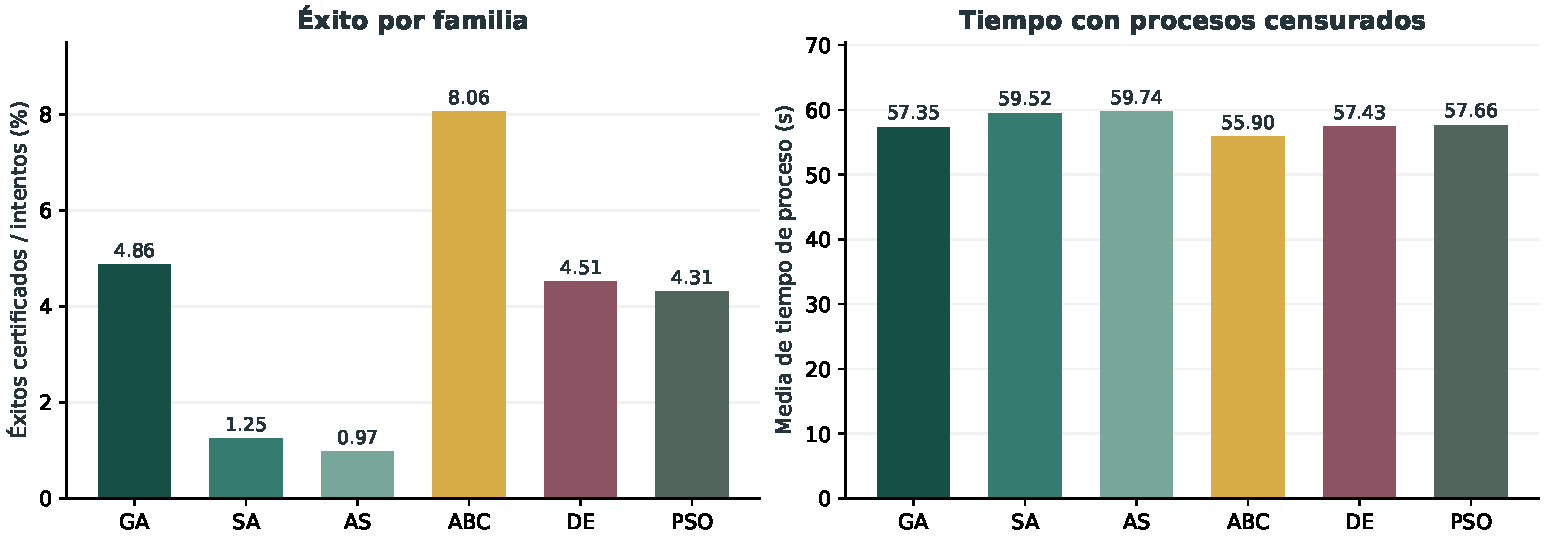
\includegraphics[width=\linewidth]{figures/performance.pdf}
\caption{Éxito y tiempo descriptivos con cobertura completa. Las medias incorporan procesos sin solución que agotaron el plazo; no equivalen a tiempos medios hasta éxito.}\label{fig:performance}
\end{figure}

Las medias están próximas al plazo por los agotamientos. Más éxitos tempranos pueden reducir la media sin implicar mayor rapidez cuando no se resuelve. Se incluyen arranque/carga y se mantienen los tiempos faltantes; la mezcla de ejecución serial y paralela impide interpretarlo como un orden de eficiencia.

\subsection{Distribución de tiempos y costos}
Las figuras~\ref{fig:timeboxes} y~\ref{fig:costboxes} complementan las medias con diagramas de cajas por familia. Se utilizan los 144 grafos completos, separando ejecución serial y paralela. Cada etiqueta indica el número de observaciones disponibles; no se imputan tiempos ni costos ausentes. Los paneles tienen subconjuntos de instancias y equipos diferentes, por lo que no son una comparación controlada entre modos.

\begin{figure}[H]\centering
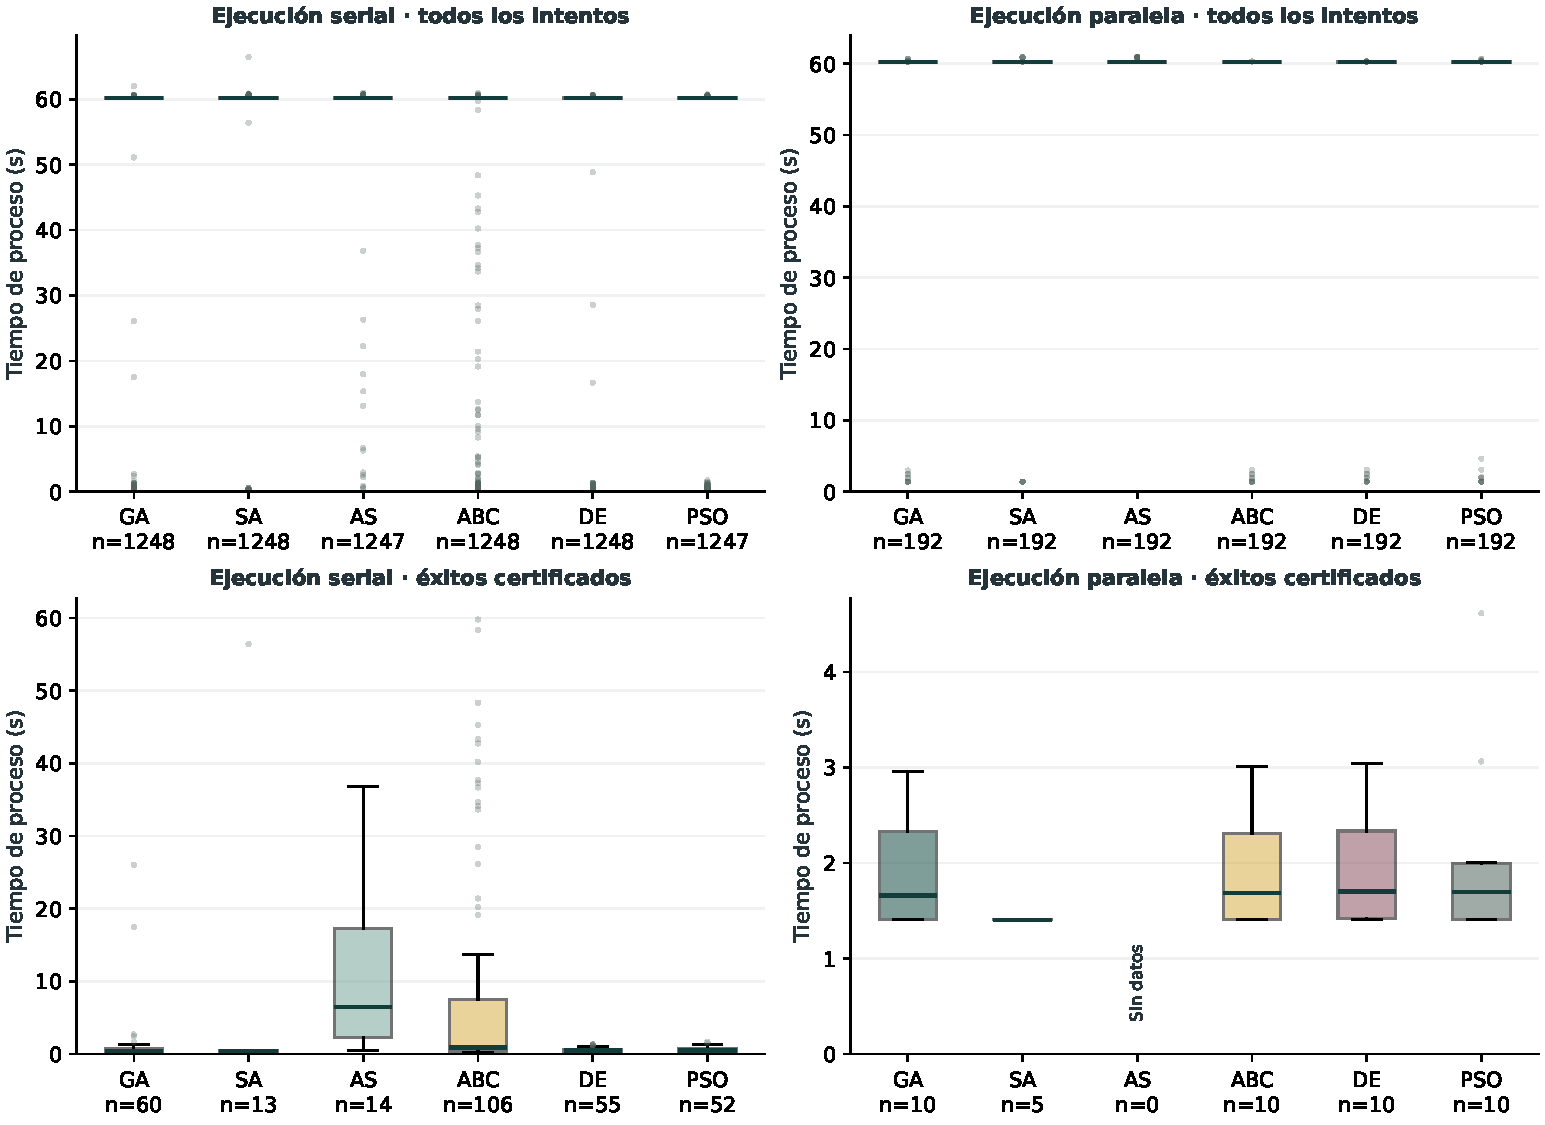
\includegraphics[width=\linewidth]{figures/runtime-boxplots.pdf}
\caption{Distribución de tiempos de proceso. Arriba: todos los intentos con duración disponible, incluidos agotamientos e incidencias. Abajo: únicamente éxitos certificados, un subconjunto condicionado a resolver. La caja abarca los percentiles 25--75, la línea indica la mediana y los bigotes llegan hasta los valores observados dentro de 1.5 rangos intercuartílicos; los puntos exteriores no se eliminan.}\label{fig:timeboxes}
\end{figure}

La concentración de cajas cerca de 60 segundos refleja el presupuesto y la censura de las búsquedas sin éxito. Los puntos rápidos pueden corresponder a soluciones tempranas o incidencias; el panel de éxitos los distingue sin convertir su distribución en tiempo general hasta solución. Una caja estrecha no demuestra robustez fuera de este corte. Los paneles vacíos indican ausencia de éxitos y no tiempo cero.

\begin{figure}[H]\centering
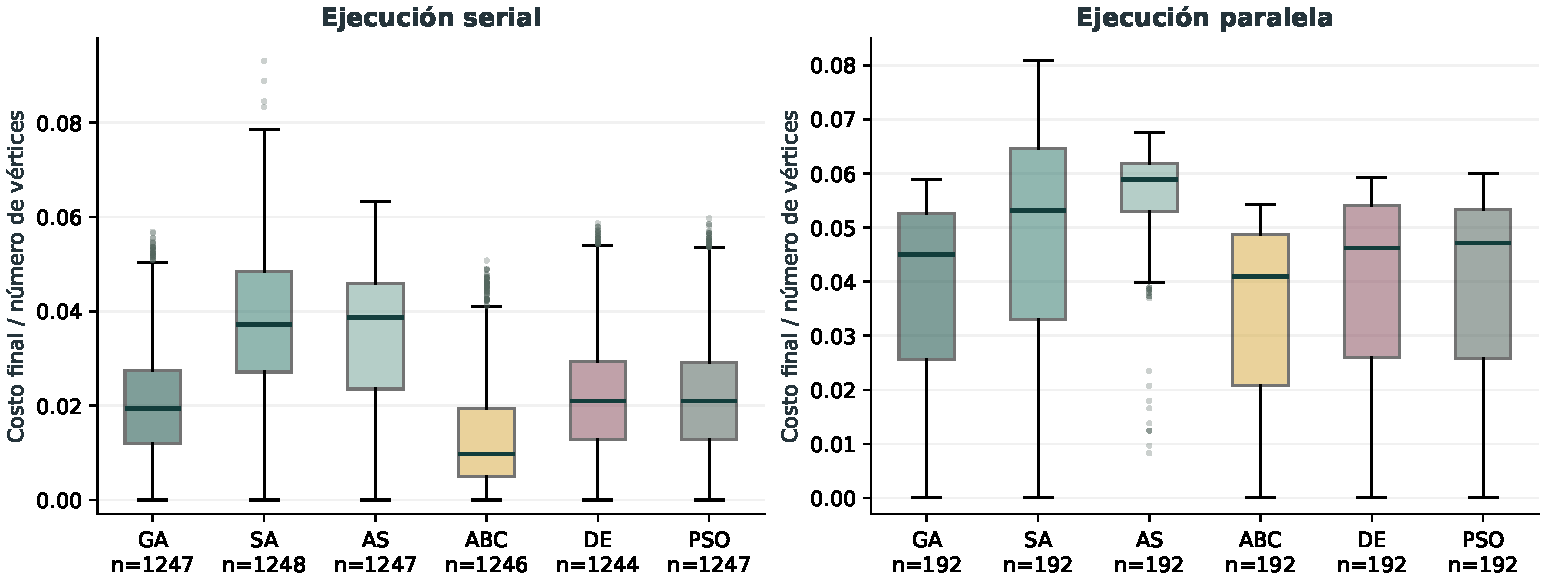
\includegraphics[width=\linewidth]{figures/cost-boxplots.pdf}
\caption{Distribución del mejor costo final por intento, dividido entre el número de vértices, con la misma convención de cajas y bigotes. Se incluyen los candidatos disponibles de los grafos completos, con y sin éxito. Un valor cero requiere además el certificado independiente.}\label{fig:costboxes}
\end{figure}

La normalización facilita mostrar grafos de tamaños distintos, pero no iguala su dificultad estructural. Un costo positivo pequeño sigue siendo una ruta sin ciclo certificado. Los cuartiles, bigotes, tamaños de muestra y cantidad de puntos exteriores se exportan en \code{docs/latex/tables/boxplot-statistics.csv}.

\subsection{Los 22 grafos certificados y variación entre semillas}
El cuadro~\ref{tab:solved} incluye los 22 grafos distintos certificados en las entregas. Para cada grafo muestra el protocolo en el que se obtuvo su primer certificado y los éxitos/intentos de esa misma evaluación. La figura~\ref{fig:heatmap} conserva ese criterio por familia y explicita los denominadores: cinco intentos en los dos grafos de la exploración guiada y diez en las otras filas. La selección y los presupuestos difieren, por lo que las celdas describen los registros y no una comparación controlada entre protocolos.

\begin{table}[H]\centering\small
\caption{Los 22 grafos distintos certificados en el conjunto de entregas. El denominador corresponde a los intentos admitidos en el protocolo indicado, incluidas incidencias; los éxitos pueden proceder de varias familias.}\label{tab:solved}
\begin{tabularx}{\linewidth}{lrYr}
\toprule
Grafo & Vértices & Protocolo del certificado & Éxitos/intentos \\ \midrule
1 & 66 & Reparación v4 30 s & 3/60 \\
2 & 70 & Distribuida 60 s & 26/60 \\
4 & 84 & Guiada 30 s & 1/30 \\
6 & 94 & Distribuida 60 s & 20/60 \\
10 & 118 & Distribuida 60 s & 13/60 \\
14 & 142 & Distribuida 60 s & 9/60 \\
18 & 166 & Distribuida 60 s & 6/60 \\
23 & 190 & Distribuida 60 s & 5/60 \\
27 & 214 & Distribuida 60 s & 6/60 \\
31 & 238 & Distribuida 60 s & 2/60 \\
35 & 262 & Guiada 30 s & 1/30 \\
39 & 286 & Reparación v4 30 s & 1/60 \\
43 & 310 & Reparación v4 30 s & 2/60 \\
47 & 334 & Reparación v4 30 s & 2/60 \\
52 & 358 & Reparación v4 30 s & 3/60 \\
56 & 382 & Distribuida 60 s & 1/60 \\
72 & 460 & Distribuida 60 s & 44/60 \\
79 & 480 & Distribuida 60 s & 43/60 \\
90 & 510 & Distribuida 60 s & 41/60 \\
96 & 540 & Distribuida 60 s & 44/60 \\
134 & 724 & Distribuida 60 s & 45/60 \\
150 & 823 & Distribuida 60 s & 40/60 \\
\bottomrule\end{tabularx}

\end{table}

\begin{figure}[H]\centering
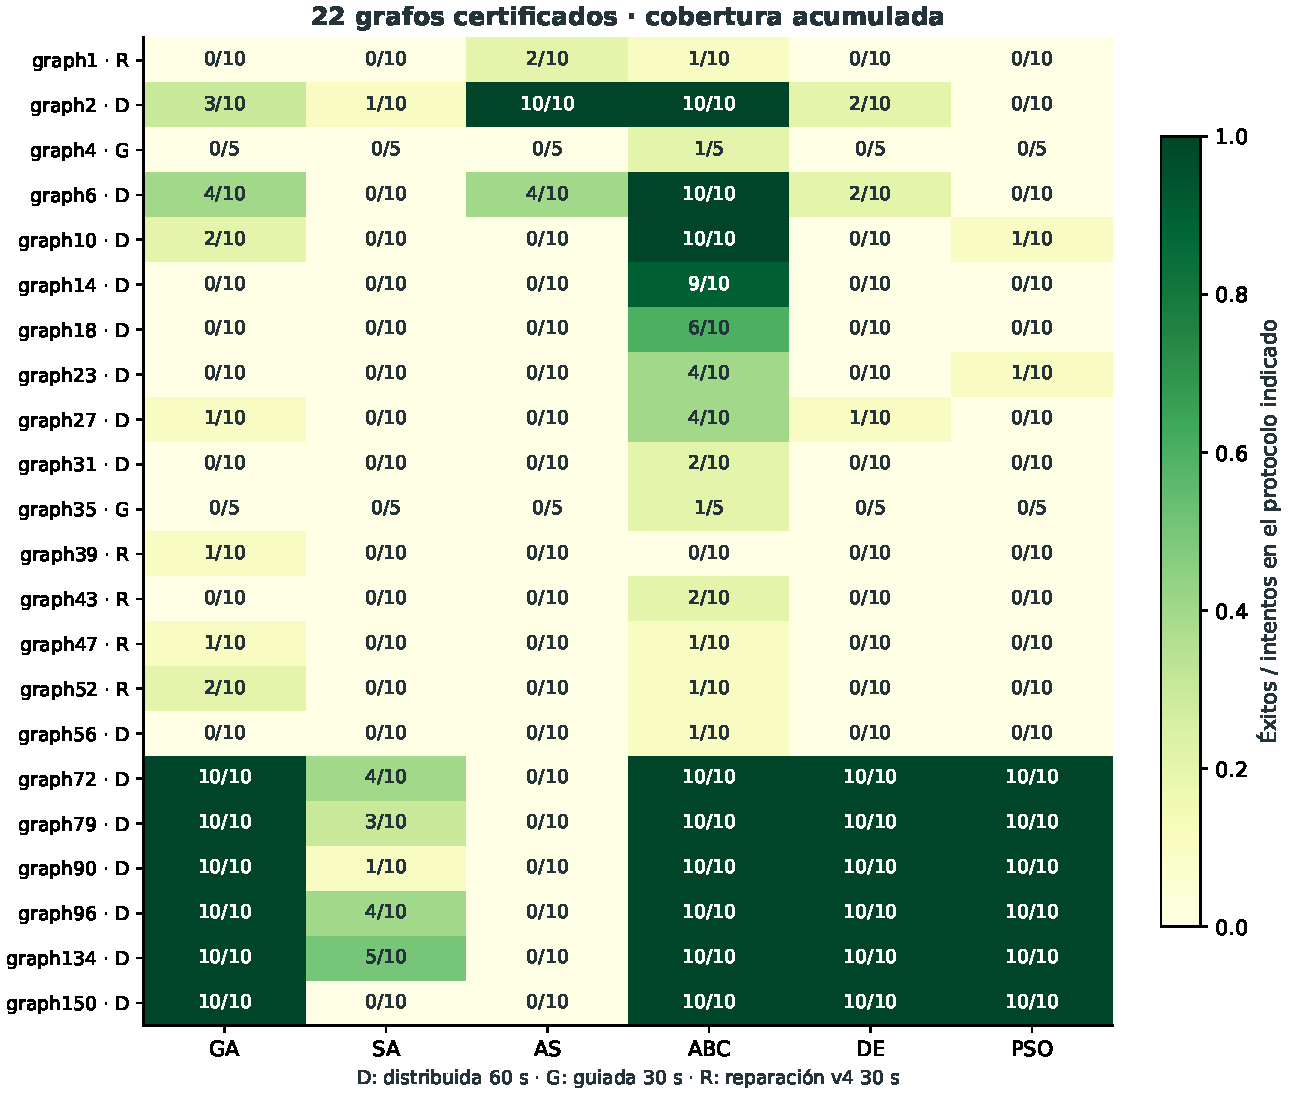
\includegraphics[width=.98\linewidth]{figures/exploratory-cumulative-heatmap.pdf}
\caption{Los 22 grafos certificados. Cada celda muestra éxitos/intentos de la familia en el protocolo indicado en la fila: D, distribuida (60 s); G, exploración guiada (30 s); R, reparación v4 (30 s). El color representa esa fracción dentro de su propio protocolo. No se mezclan intentos de configuraciones distintas ni se extrapola al challenge completo.}\label{fig:heatmap}
\end{figure}

\subsection{Calidad de candidatos y escala}
La figura~\ref{fig:cost} muestra el menor costo normalizado observado por grafo iniciado en cualquiera de las tres entregas, incluidos los resultados recientes. Los 22 grafos certificados aparecen en cero; los valores positivos indican transiciones ausentes. Un costo pequeño puede significar cercanía en esta función objetivo y, aun así, no cumplir el cierre. El eje de vértices se presenta en escala logarítmica para conservar legibilidad entre tamaños.

\begin{figure}[H]\centering
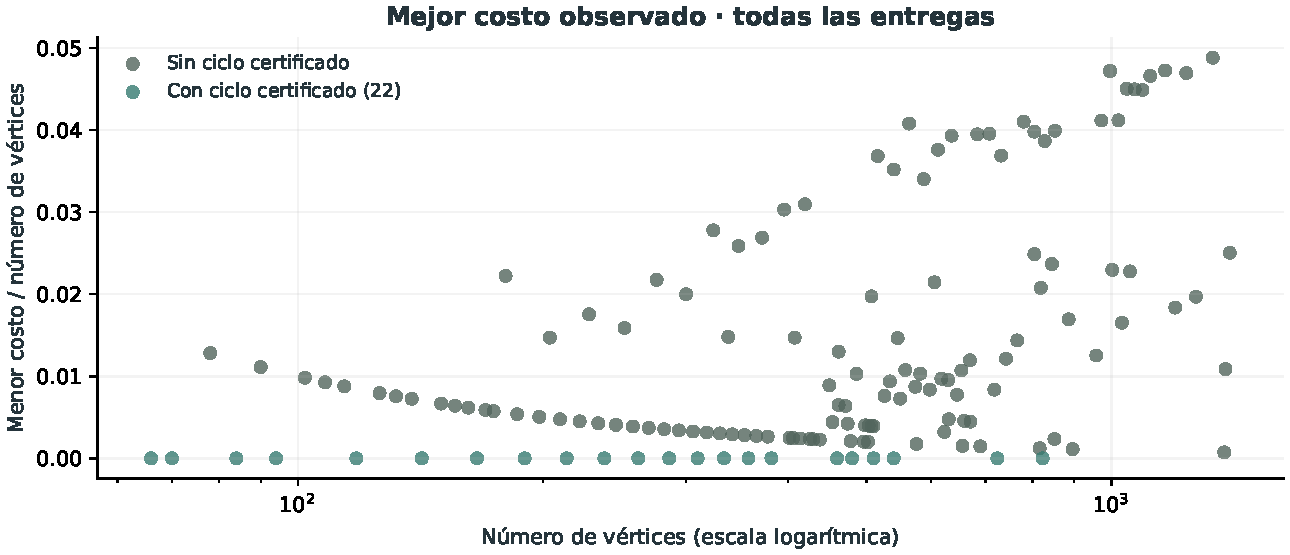
\includegraphics[width=\linewidth]{figures/exploratory-cumulative-cost.pdf}
\caption{Mejor costo acumulado entre las entregas para los 149 grafos iniciados, con 22 ciclos certificados. Se toma el mínimo disponible por ID sin sumar costos ni equiparar presupuestos; las instancias tienen distinta cobertura de intentos y configuraciones.}\label{fig:cost}
\end{figure}

La figura no identifica causalidad: tamaño, estructura, hardware, políticas y cobertura cambian conjuntamente. No se extrapola a los 852 grafos sin iniciar.

\subsection{Incidencias preservadas}
Se preservaron tres interrupciones de Arturo, seis de Zapata, dos de César y una de Eder, sin reintentos automáticos. Los 600 primarios de Elías pudieron recuperarse y auditarse pese al fallo de longitud de ruta y los huecos de su historial de sesiones.
